%----------------------------------------------------------------------------------------
%	PACKAGES AND THEMES
%----------------------------------------------------------------------------------------

\documentclass[11.5pt, aspectratio=169]{beamer} %handout

\usepackage{Style/style}

%----------------------------------------------------------------------------------------
%	TITLE PAGE
%----------------------------------------------------------------------------------------

% The short title appears at the bottom of every slide, the full title is only on the title page
\title[]{Exploration in Policy Search by Multiple Importance Sampling} 

\author[L.\,Lupo]
{%
  \texorpdfstring{
    \begin{columns}%[onlytextwidth]
      \column{1\linewidth}
      \centering
      Lorenzo Lupo\\
      \href{mailto:lorenzo.lupo@mail.polimi.it}{lorenzo.lupo@mail.polimi.it}
    \end{columns}
  }
  {Lorenzo Lupo}
}
		 
\institute[Polimi] % Your institution as it will appear on the bottom of every slide, may be shorthand to save space
{%
%Politecnico di Milano%\\ % Your institution for the title page
%\medskip
%\textit{john@smith.com} % Your email address
}
\date{April 16th, 2019}

\begin{document}

\begin{frame}[plain]
	\begin{figure}[htpb]
		\centering
		
\includegraphics[width=0.3\linewidth]{Images/polimi}
	\end{figure}
	\titlepage
\end{frame}

%------------------------------------------------------------------------------
% Introduzione 
%------------------------------------------------------------------------------

\begin{frame}{How can robots learn to backflip?}

	\begin{figure}
		\centering
		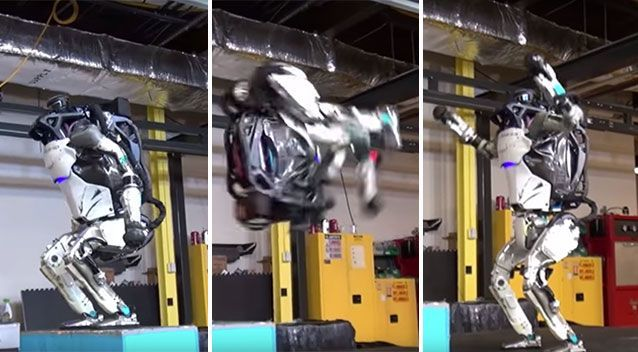
\includegraphics[width=0.7\linewidth]{Images/atlas}
	\end{figure}
\end{frame}

%https://giphy.com/gifs/boston-atlas-dynamic-riIyHZrGO0aju


\begin{frame}{Algorithmic Trading}
	\begin{figure}
		\centering
		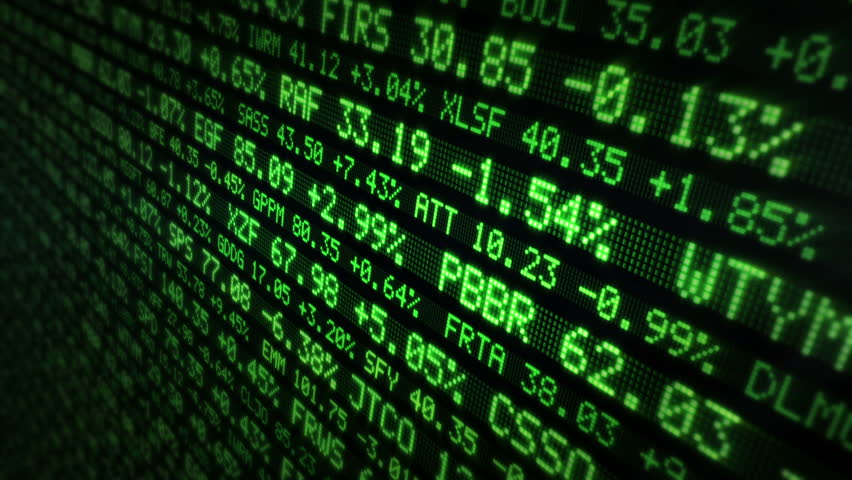
\includegraphics[width=0.7\linewidth]{Images/stocks}
	\end{figure}
\end{frame}

\begin{frame}{Self-driving Cars}
	\begin{figure}
		\centering
		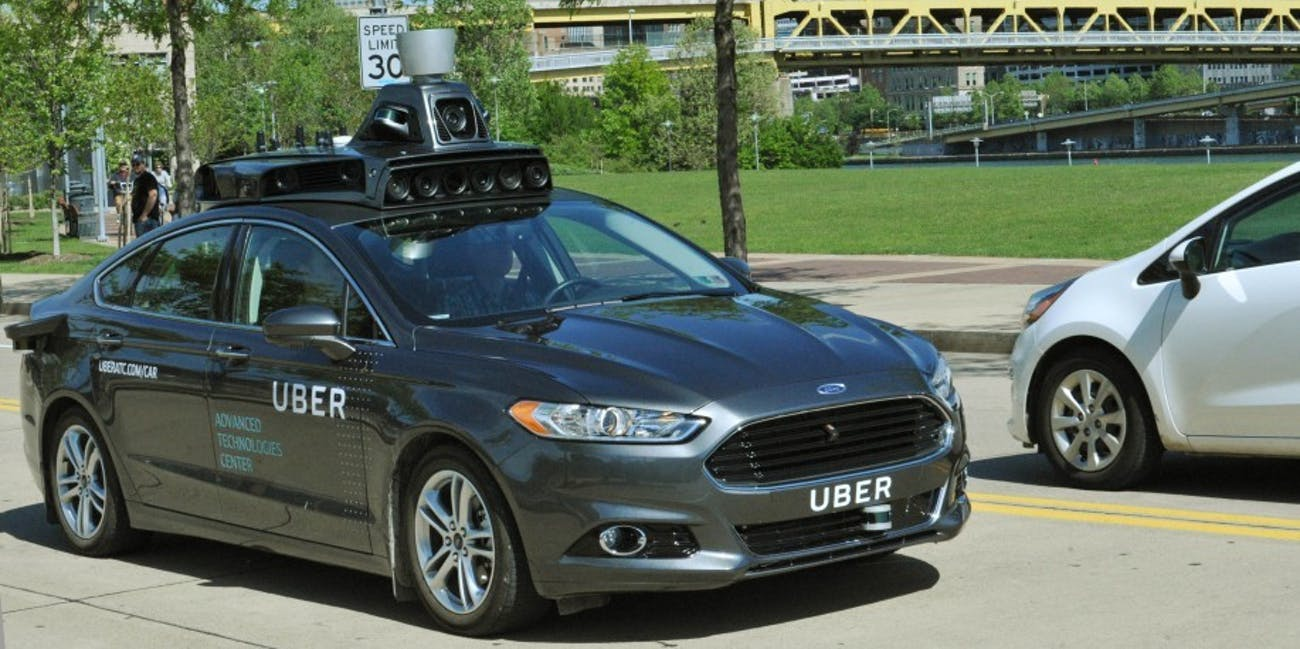
\includegraphics[width=0.7\linewidth]{Images/uber}
	\end{figure}
\end{frame}

%\begin{frame}{The Computerization of Finance}
%	\begin{figure}
%		\centering
%		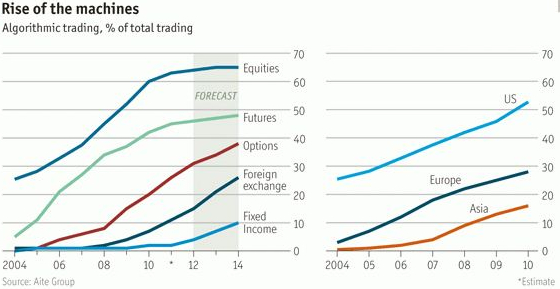
\includegraphics[width=0.7\linewidth]{Images/2_algo_trading}
%	\end{figure}
%\end{frame}




%------------------------------------------------------------------------------
% Indice 
%------------------------------------------------------------------------------

%\begin{frame}
%\frametitle{Plan} % Table of contents slide, comment this block out to remove it
%\tableofcontents % Throughout your presentation, if you choose to use \section{} and \subsection{} commands, these will automatically be printed on this slide as an overview of your presentation
%\end{frame}

%------------------------------------------------------------------------------
% Corpo della presentazione 
%------------------------------------------------------------------------------

\section{Basics of Reinforcement Learning}
\label{sec:reinforcement_learning}

\begin{frame}{The Reinforcement Learning Framework}
\begin{figure}[t]
	\centering
	\begin{tikzpicture}[node distance = 6em, auto, thick]
		\onslide<2->{%
			\node at (4, 0) (Environment) {
\includegraphics[width=3cm]{Images/environment}};
			\node at (4, 2) {\LARGE Environment};
			\node at (4, -2) {\LARGE $\calP$, $\calR$};
		}
		
		\onslide<3->{%
			\node at (-4, 0) (Agent) {
\includegraphics[width=3cm]{Images/agent}};
			\node at (-4, 2) {\LARGE Agent};
			\node at (-4, -2) {\LARGE $\pi$};
		}
		
		\onslide<4->{%
		\draw [->, line width=5pt, MyLightGreen, opacity=0.7] (Environment) to [bend right=35] (Agent);
		\node at (0, 2.5) {\Large State $s_h$};
		}
		
		\onslide<5|handout:0>{%
		\node[draw=MyLightGreen, opacity=0.7, circle, line width=3pt, minimum size=1cm] at (-4, -2) {};
		}
		
		\onslide<6->{%
		\draw [->, line width=5pt, MyLightGreen, opacity=0.7] (Agent) to [bend right=35] (Environment);
		\node at (0, -2.5) {\Large Action $a_h$};
		}
		
		\onslide<7|handout:0>{%
		\node[draw=MyLightGreen, opacity=0.7, circle, line width=3pt, minimum size=1cm] at (3.56, -2) {};	
		}
		
		\onslide<8|handout:0>{%
		\node[draw=MyLightGreen, opacity=0.7, circle, line width=3pt, minimum size=1cm] at (4.42, -2) {};	
		}
					
		\onslide<9->{%
		\draw [->, line width=5pt, MyLightGreen, opacity=0.7] (Environment) to (Agent);
		\node at (0, 0.5) {\Large Reward $r_{h+1}$};
		}		
	\end{tikzpicture}
\end{figure}
\end{frame}

\begin{frame}{Policy Search Formulation}

	\onslide<1->{%
	\textbf{Cumulative return of a trajectory $\tau$:}
		\begin{equation*}
		\Rew(\tau) = \sum_{h=0}^{H-1}\gamma^hr_{h+1},\text{ with } \tau=[s_0,a_0,s_1,a_1,\dots,s_{H-1},a_{H-1}]
		\end{equation*}
	}

	\onslide<2->{%
	\textbf{Parametric policy:}
		\begin{equation*}
		\pi_{\vtheta}:\Sspace\to\Delta(\Aspace),\text{ \ie \,}\pi_{\vtheta}(a|s) = \frac{1}{\sqrt{2\pi}\sigma}\exp\left(-\frac{1}{2}\left(\frac{a-\vtheta^T\phi(s)}{\sigma}\right)^2\right)
		\end{equation*}
	}
	
	\onslide<3->{%
	\textbf{Performance:}
		\begin{equation*}
		\mu(\vtheta) = \Exp_{\tau\sim p_{\vtheta}}[\Rew(\tau)],\text{ where } p_{\vtheta} \text{ is the \textbf{distribution over trajectories} } \tau\in\Tau\text { induced by } \pi_{\vtheta}
		\end{equation*}
	}

	
	\onslide<4->{%
	\textbf{Objective:}
		\begin{equation*}
\vtheta^* = \arg \max_{\vtheta\in\Theta}\mu(\vtheta).
\end{equation*}
	}
	
\end{frame}

\begin{frame}{Exploration VS Exploitation}
	\begin{figure}
		\centering
		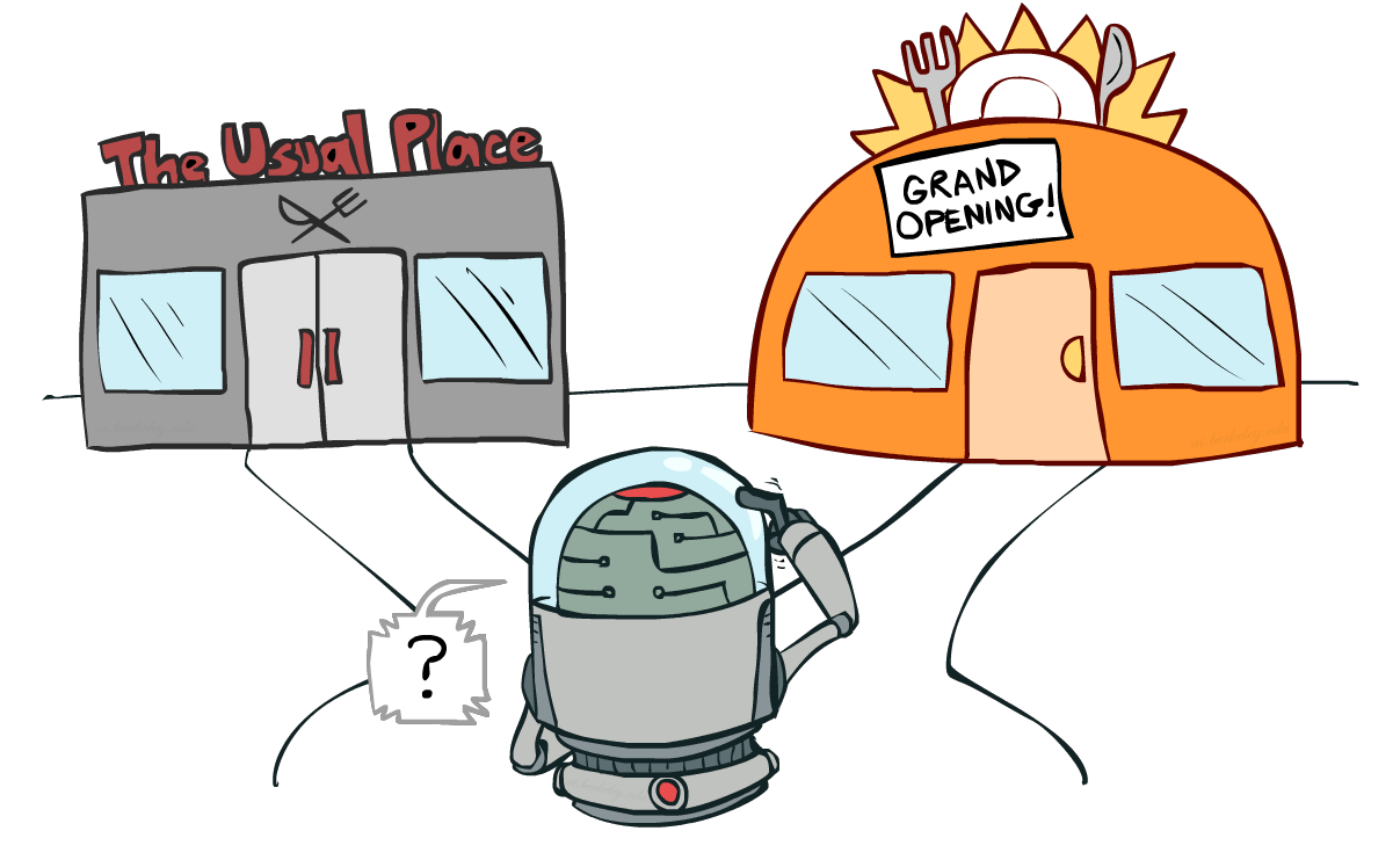
\includegraphics[width=0.7\linewidth]{Images/exp_exp}
	\end{figure}
\end{frame}

%\begin{frame}{Taxonomy of RL Algorithms}
%\begin{figure}[t]
%	\centering
%	\begin{tikzpicture}[node distance = 6em, auto, thick]
%		
%		\onslide<1->{%
%			\node [draw=LightSteelBlue, circle, line width=5pt, minimum size=2cm] at (-4, 0) (Model) {\Large $\calP$, $\calR$};
%			\node at (-4, 1.5) {\Large Model};
%		}
%		
%		\onslide<2->{%
%			\node [draw=SteelBlue, circle, line width=5pt, minimum size=2cm] at (-0, 0) (Value) {\Large $V_*$, $Q_*$};
%			\node at (0, 1.5) {\Large Value Functions};
%			\draw [->, line width=5pt, LightGray] (Model) to (Value);
%		}
%
%		\onslide<3->{%
%			\node [draw=Blue, circle, line width=5pt, minimum size=2cm] at (4, 0) (Policy) {\Large $\pi_*$};
%			\node at (4, 1.5) {\Large Policy};
%			\draw [->, line width=5pt, LightGray] (Value) to (Policy);
%		}
%		
%		\onslide<4->{%
%			\node [draw=LightSteelBlue, circle, line width=5pt, minimum size=2cm] at (-4, -3) (ApproxModel) {\Large $\widehat{\calP}$, $\widehat{\calR}$};
%			\node at (-4, -4.5) {\Large Model-Based};
%			\draw [dashed, line width=5pt, LightGray] (ApproxModel) to (Model);
%		}
%		
%		\onslide<5->{%
%			\node [draw=SteelBlue, circle, line width=5pt, minimum size=2cm] at (0, -3) (ApproxValue) {\Large $\widehat{V}$, $\widehat{Q}$};
%			\node at (0, -4.5) {\Large Value-Based};
%			\draw [dashed, line width=5pt, LightGray] (ApproxValue) to (Value);
%		}
%		
%		\onslide<6->{%
%			\node [draw=Blue, circle, line width=5pt, minimum size=2cm] at (4, -3) (ApproxPolicy) {\Large $\widehat{\pi}$};
%			\node at (4, -4.5) {\Large Policy-Based};
%			\draw [dashed, line width=5pt, LightGray] (ApproxPolicy) to (Policy);
%		}
%	\end{tikzpicture}
%\end{figure}
%\end{frame}
%
%
%
%

\section{Exploration in Policy Search}


\begin{frame}{Exploration in Policy Search}
	
	\begin{block}{Undirected exploration}
	Explore actions based on randomness, without any knowledge of the learning process.

	\begin{itemize}[noitemsep,topsep=0pt]
		\item<+(1)-|alert@+(1)> E.g.1: by adopting stochastic policies \cite{deisenroth2013survey}.
		\item<+(1)-|alert@+(1)> E.g.2: by augmenting rewards with the entropy of the policy \cite{haarnoja2018soft}: 
		\begin{equation*}
		\Rew(\tau) = \sum_{h=0}^{H-1}\gamma^hr_{h+1} + \mathcal{H}(\pi_{\vtheta}(\cdot|s_h)).
		\end{equation*}
	\end{itemize}
	\end{block}
	
	\onslide<+(1)->{
	\begin{block}{Directed exploration}
	Leverage on the knowledge acquired during learning.
		\begin{itemize}
		\item<+(1)|alert@+(1)-> E.g.: Count-based techniques \cite{bellemare2016unifying}.
		\end{itemize}
	\end{block}
	}
	
\end{frame}

%\begin{frame}{Exploration in Policy Search}
%	
%	\begin{block}{Undirected exploration}
%	\begin{enumerate}
%		\item<+-> Adding noise to action selection by adopting stochastic policies;
%		\item<+-> Augmenting the reward with entropy 
%		\begin{equation*}
%		\theta_{k+1} = \theta_k + \alpha_k 
%       		\tikz[baseline]{
%           		\node[anchor=base] (gradient) {$\nabla_\theta J\left(\theta_k\right)$};
%       	   }
%		\end{equation*}
%	\end{enumerate}
%	\end{block}
%	
%	\onslide<+-|handout:0>{
%		\begin{tikzpicture}[overlay]
%				\node[draw=SteelBlue, circle, line width=3pt, minimum size=1.8cm] at (8.67, 1.65) (g) {};
%				\node[SteelBlue] at (11,-0.2) (q) {\Huge \textbf{?}};
%		        \draw [->, line width=3pt, SteelBlue] (q) to [bend left=35] (g);
%		\end{tikzpicture}
%	}
%\end{frame}

%\begin{frame}{The Keystone of Policy Gradient Algorithms}
%	
%	\onslide<1->
%	\begin{alertblock}{Policy Gradient Theorem}
%		\begin{equation*}
%			\nabla_\theta J(\theta) =
%			\E[\substack{S \sim d^\theta\\A \sim \pi_\theta}]{\nabla_\theta\log
%			\pi_\theta(S,A) Q_{\theta}(S, A)}
%		\end{equation*}
%	\end{alertblock}
%	
%	\onslide<2->{
%	For an episodic environment, the policy gradient can be approximated via Monte-Carlo
%	\begin{equation*}
%		\nabla_\theta J(\theta_k) \approx \frac{1}{M} \sum_{m=0}^M
%		 \sum_{u=0}^{T^{(m)}-1} \nabla_\theta\log \pi_{\theta_k} \left(s_u^{(m)}, a_u^{(m)}\right) \sum_{v \geq u}^{T^{(m)}-1} \gamma^{v-u} r_{v+1}^{(m)}   
%	\end{equation*}
%	}
%	
%	\onslide<3->{
%		However, this estimate is characterized by a large variance. Possible improvements:
%		\begin{enumerate}
%			\item Optimal baseline
%			\item Actor-critic methods
%			\item Natural gradient
%		\end{enumerate}
%	}
%\end{frame}
%
%\begin{frame}{Policy Gradient with Parameter-Based Exploration (PGPE)}
%	\begin{block}{Key Idea}
%		\begin{enumerate}
%			\item<+-> Actions are selected using a deterministic parametric controller $F_\theta$
%			\item<+-> The controller parameters are drawn from a probability distribution $p_\xi$
%			\item<+-> The search for an optimum is performed in the space of the hyperparameters $\xi$
%		\end{enumerate}
%	\end{block}
%	
%	\onslide<+->{
%		More formally, the update scheme becomes
%			\begin{equation*}
%				\xi_{k+1} = \xi_k + \alpha_k \nabla_\xi J(\xi_k)
%			\end{equation*}
%		where the policy gradient is given by
%		\begin{alertblock}{Parameter-Based Policy Gradient Theorem}
%			\begin{equation*}
%				\nabla_\xi J(\xi) = \E[\substack{S \sim d^\xi\\\theta \sim p_\xi}]{\nabla_\xi \log p_\xi(\theta) Q_{\xi}\left(S, F_\theta(S)\right)}
%			\end{equation*}		
%		\end{alertblock}
%	}
%\end{frame}



\section{OPTIMIST}

\begin{frame}{Problem Formulation}

\onslide<+->\begin{block}{Decision Set or Arms Set}
The parameter space $\Theta\subseteq\Reals^d$.
\end{block}

\onslide<+->\begin{block}{Procedure}
At every decision step $t\in[0,1,2,\dots,T]$:
	\begin{enumerate}
			\item<+-> \textbf{Select} an arm $\vtheta_t\in\Theta$;
			\item<+-> \textbf{Sample} a trajectory $\tau_t\in\Tau$ by following $\pi_{\vtheta_t}$;
			\item<+-> \textbf{Observe} the cumulative return $\Rew(\tau_t)$.
		\end{enumerate}
\end{block}

\onslide<+->\begin{block}{Goal}
\begin{itemize}
\item \textbf{Minimize} $Regret(T) = \sum_{t=0}^{T}\mu(\vtheta^*)-\mu(\vtheta_t)$, where $\vtheta^*=\arg\max_{\vtheta\in\Theta}\mu(\vtheta)$
\end{itemize}
\end{block}

%\onslide<+->\begin{block}{Goal}
%\begin{itemize}
%\item Maximize the total expected return $\sum_{t=0}^T \Exp_{\tau_t\sim p_{\vtheta_t}}[\Rew(\tau_t)] = \sum_{t=0}^T \mu(\vtheta)$
%\item<+-> Alternatively, minimize \textbf{regret}.
%\end{itemize}
%\end{block}

\end{frame}


\begin{frame}{Regret}

\onslide<+->\begin{block}{Decision Set or Arms Set}
The parameter space $\Theta\subseteq\Reals^d$.
\end{block}

\end{frame}

%	\onslide<2->{
%	\textbf{Rewards}: portfolio log-return with transaction costs
%		\begin{equation*}
%			R_{t+1} = \log \left\{ 1 + \sum^{I}_{i=0} \left[ 
%				\tikz[baseline]{
%		        	\node[anchor=base] (t1) {$a_t^i X_{t+1}^i$};
%		        } - 
%		        \tikz[baseline]{
%		        	\node[anchor=base] (t2) {$\delta_i \left| a_t^i - \widetilde{a}_t^i \right|$};
%		       	} -
%		       	\tikz[baseline]{
%		       		\node[anchor=base] (t3) {$\delta_s {(a_t^i)}^-$};
%		       	} \right] -
%		       	\tikz[baseline]{
%		       		\node[anchor=base] (t4) {$\delta_f \mathbf{1}_{{a}_t \neq \tilde{{a}}_{t-1}}$};
%		       	} \right\}	 	
%		 \end{equation*}
%	}
%	
%	\onslide<7->{
%	\textbf{Actions}: Portfolio weights
%		\begin{equation*}
%			\{a_t^i\}_{i=0}^I \;\;\; \text{s.t.}\;\;\; \sum^{I}_{i=0} a_t^i = 1 \;\;\;\;\; \forall t \in \{0, 1, 2, \ldots\}
%		\end{equation*}
%	}
%
%	\onslide<8->{
%	\textbf{States}: assets past returns and current allocation
%		\begin{equation*}
%			S_t = \{X, X_t, X_{t-1}, \ldots, X_{t-P}, \tilde{a}_t\}
%		\end{equation*}
%	}
%	
%	\onslide<3|handout:0>{
%		\begin{tikzpicture}[overlay]
%				\node[draw=SteelBlue, circle, line width=3pt, minimum size=2cm] at (t1) {};
%		\end{tikzpicture}
%	}
%	
%	\onslide<4|handout:0>{
%		\begin{tikzpicture}[overlay]
%				\node[draw=SteelBlue, circle, line width=3pt, minimum size=2cm] at (t2) {};
%		\end{tikzpicture}
%	}
%		
%	\onslide<5|handout:0>{
%		\begin{tikzpicture}[overlay]
%				\node[draw=SteelBlue, circle, line width=3pt, minimum size=2cm] at (t3) {};
%		\end{tikzpicture}
%	}
%			
%	\onslide<6|handout:0>{
%		\begin{tikzpicture}[overlay]
%				\node[draw=SteelBlue, circle, line width=3pt, minimum size=2cm] at (t4) (g) {};
%		\end{tikzpicture}
%	}
%\end{frame}
%
%\begin{frame}[c]{Synthetic Asset: Convergence}
%\begin{figure}[t!]
%	\centering
%	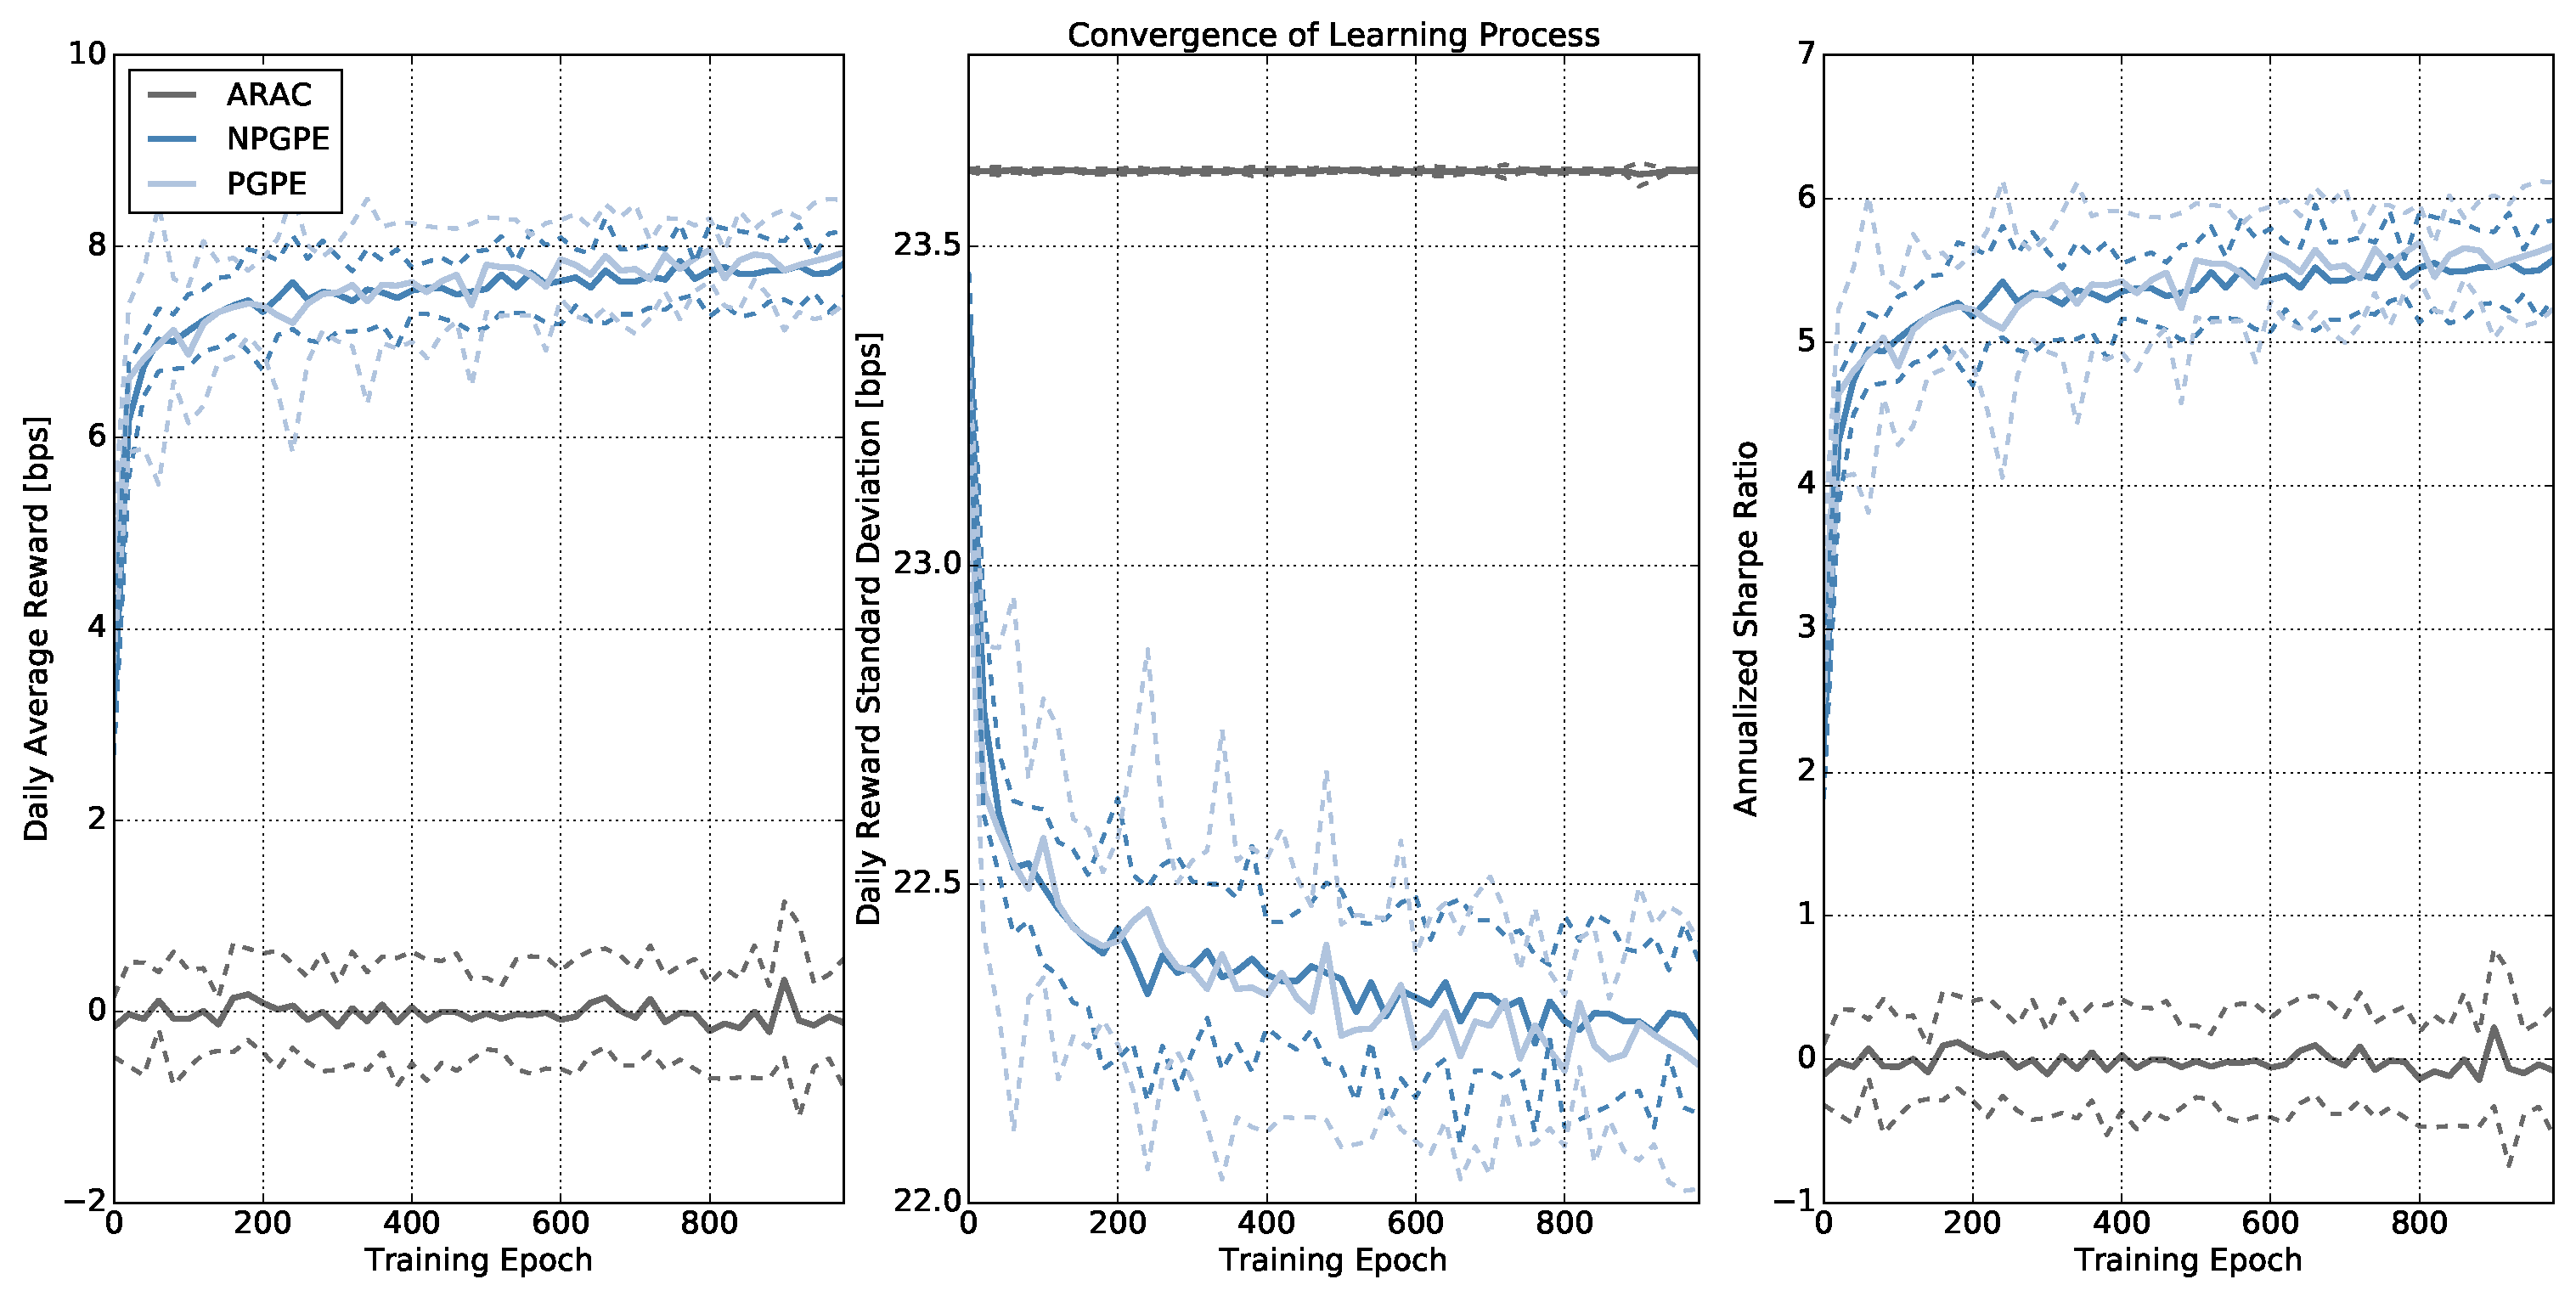
\includegraphics[height=5cm,width=0.8\textwidth]{Images/6_0_single_synthetic_neutral_convergence}
%\end{figure}
%\end{frame}
%
%
%\begin{frame}[c]{Synthetic Asset: Backtest Performance}
%\begin{figure}[t]
%	\centering
%	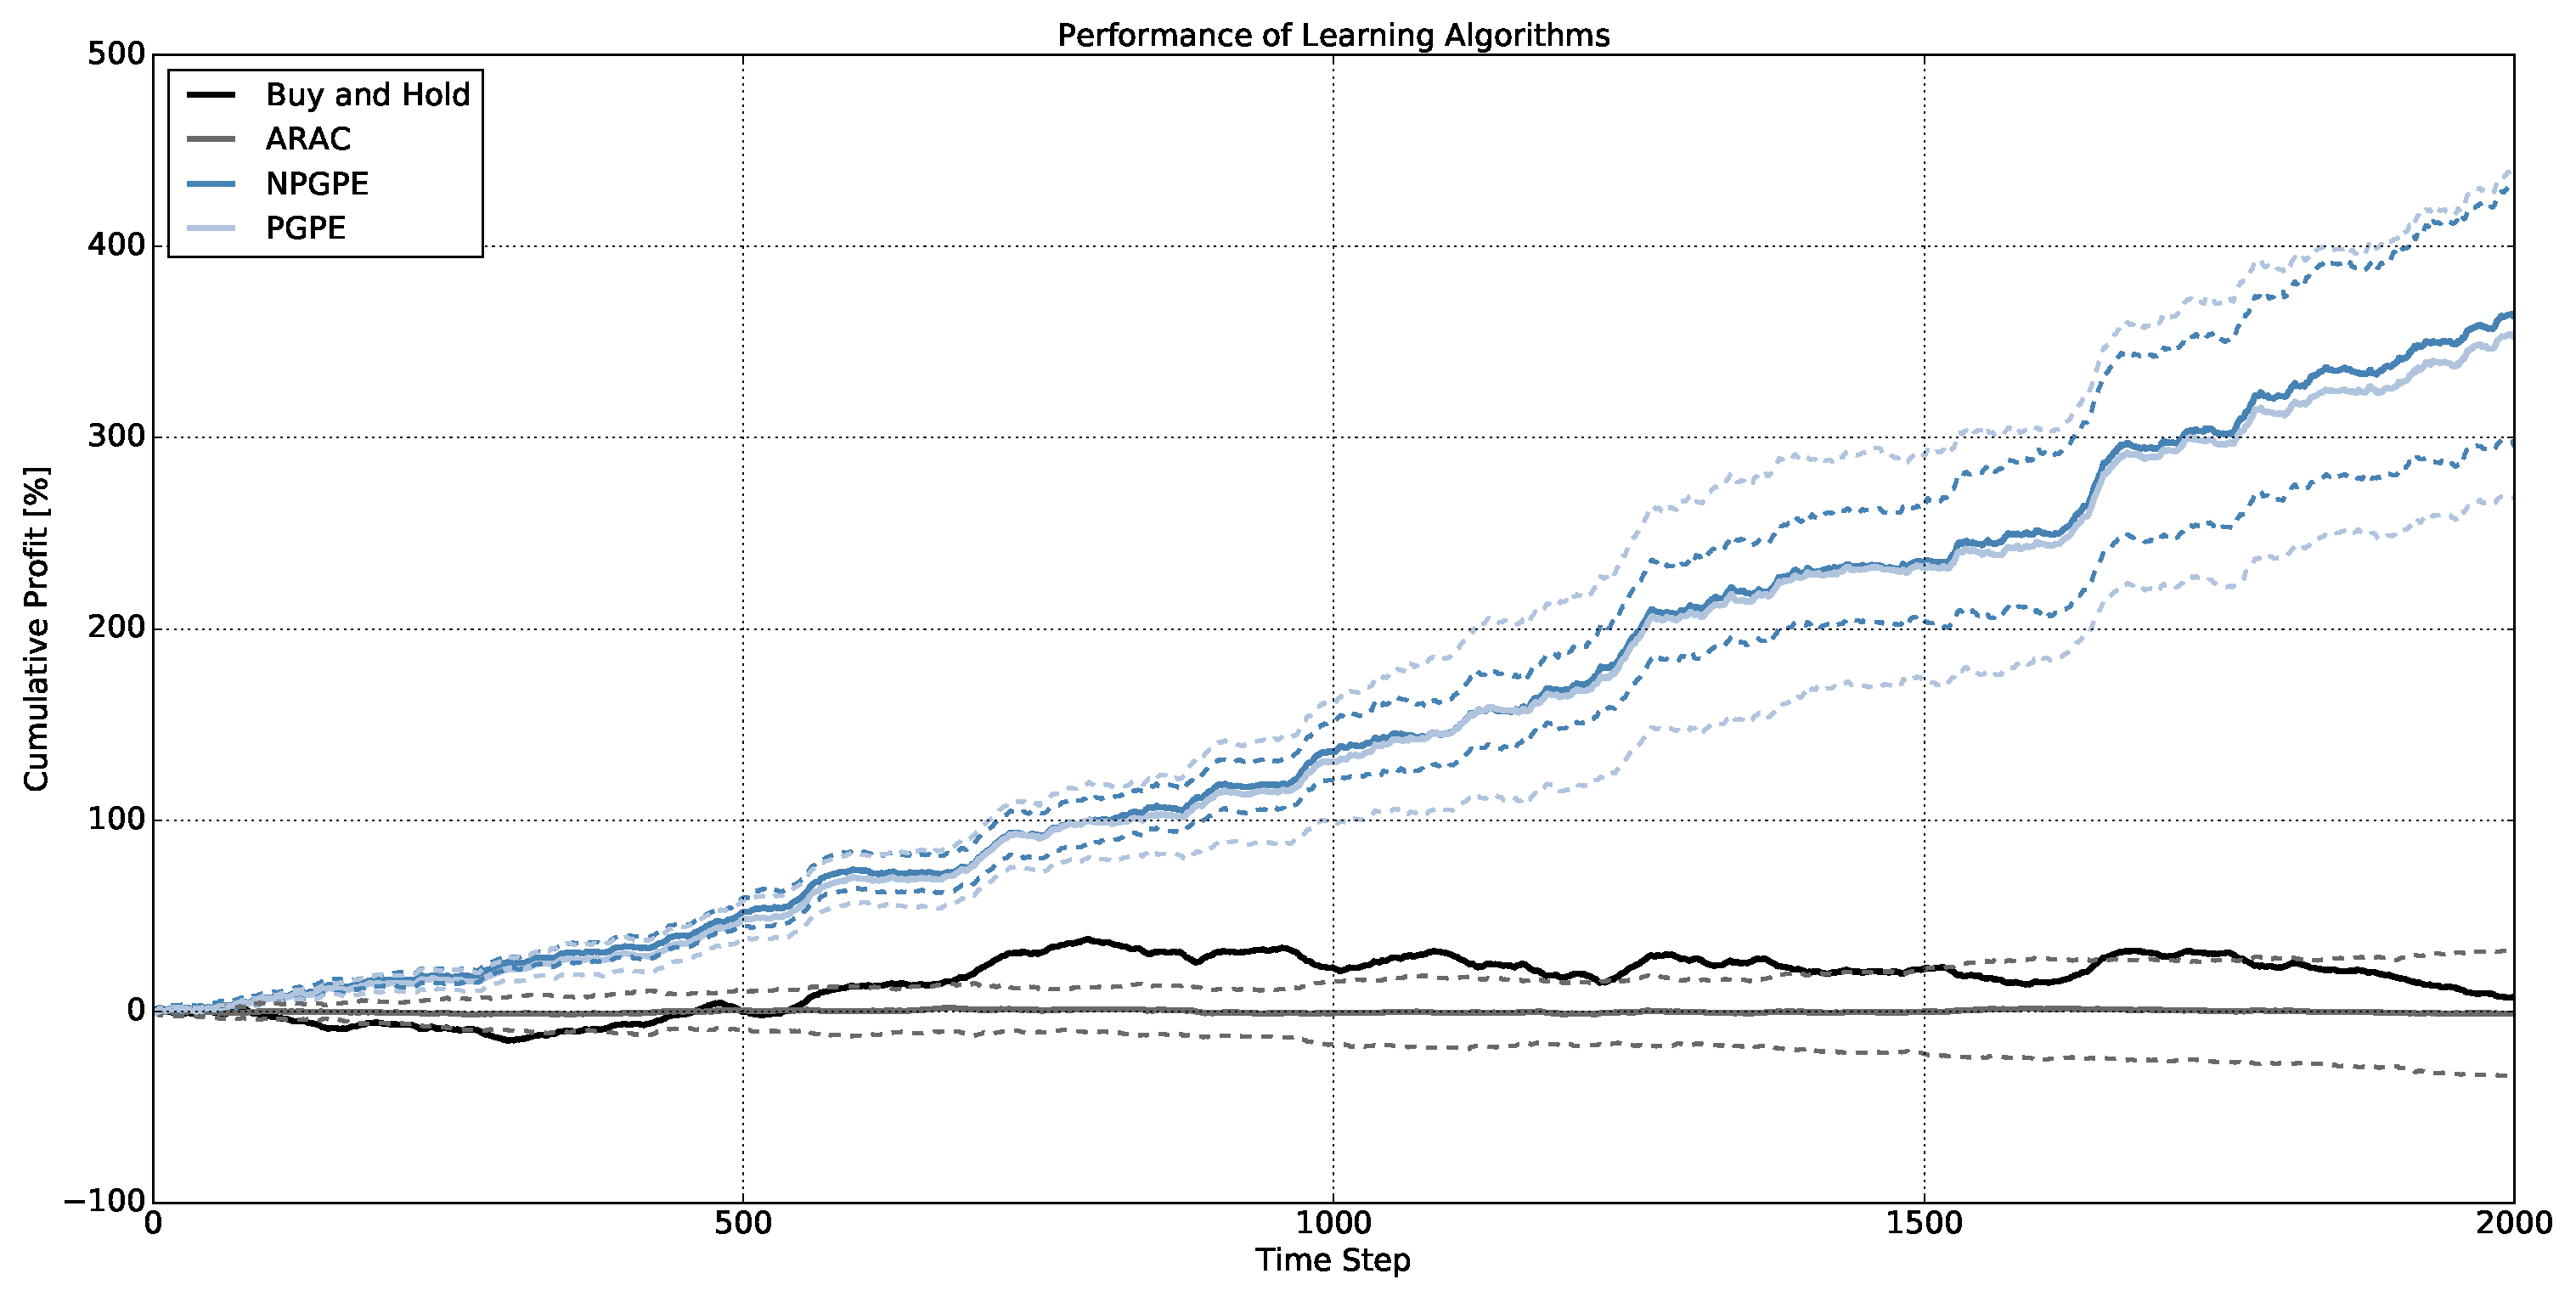
\includegraphics[height=6cm,width=0.8\textwidth]{Images/6_1_single_synthetic_neutral_performance}
%\end{figure}
%\end{frame}
%
%\begin{frame}[c]{Synthetic Asset: Impact of Transaction Costs}
%\begin{figure}[t!]
%	\centering
%	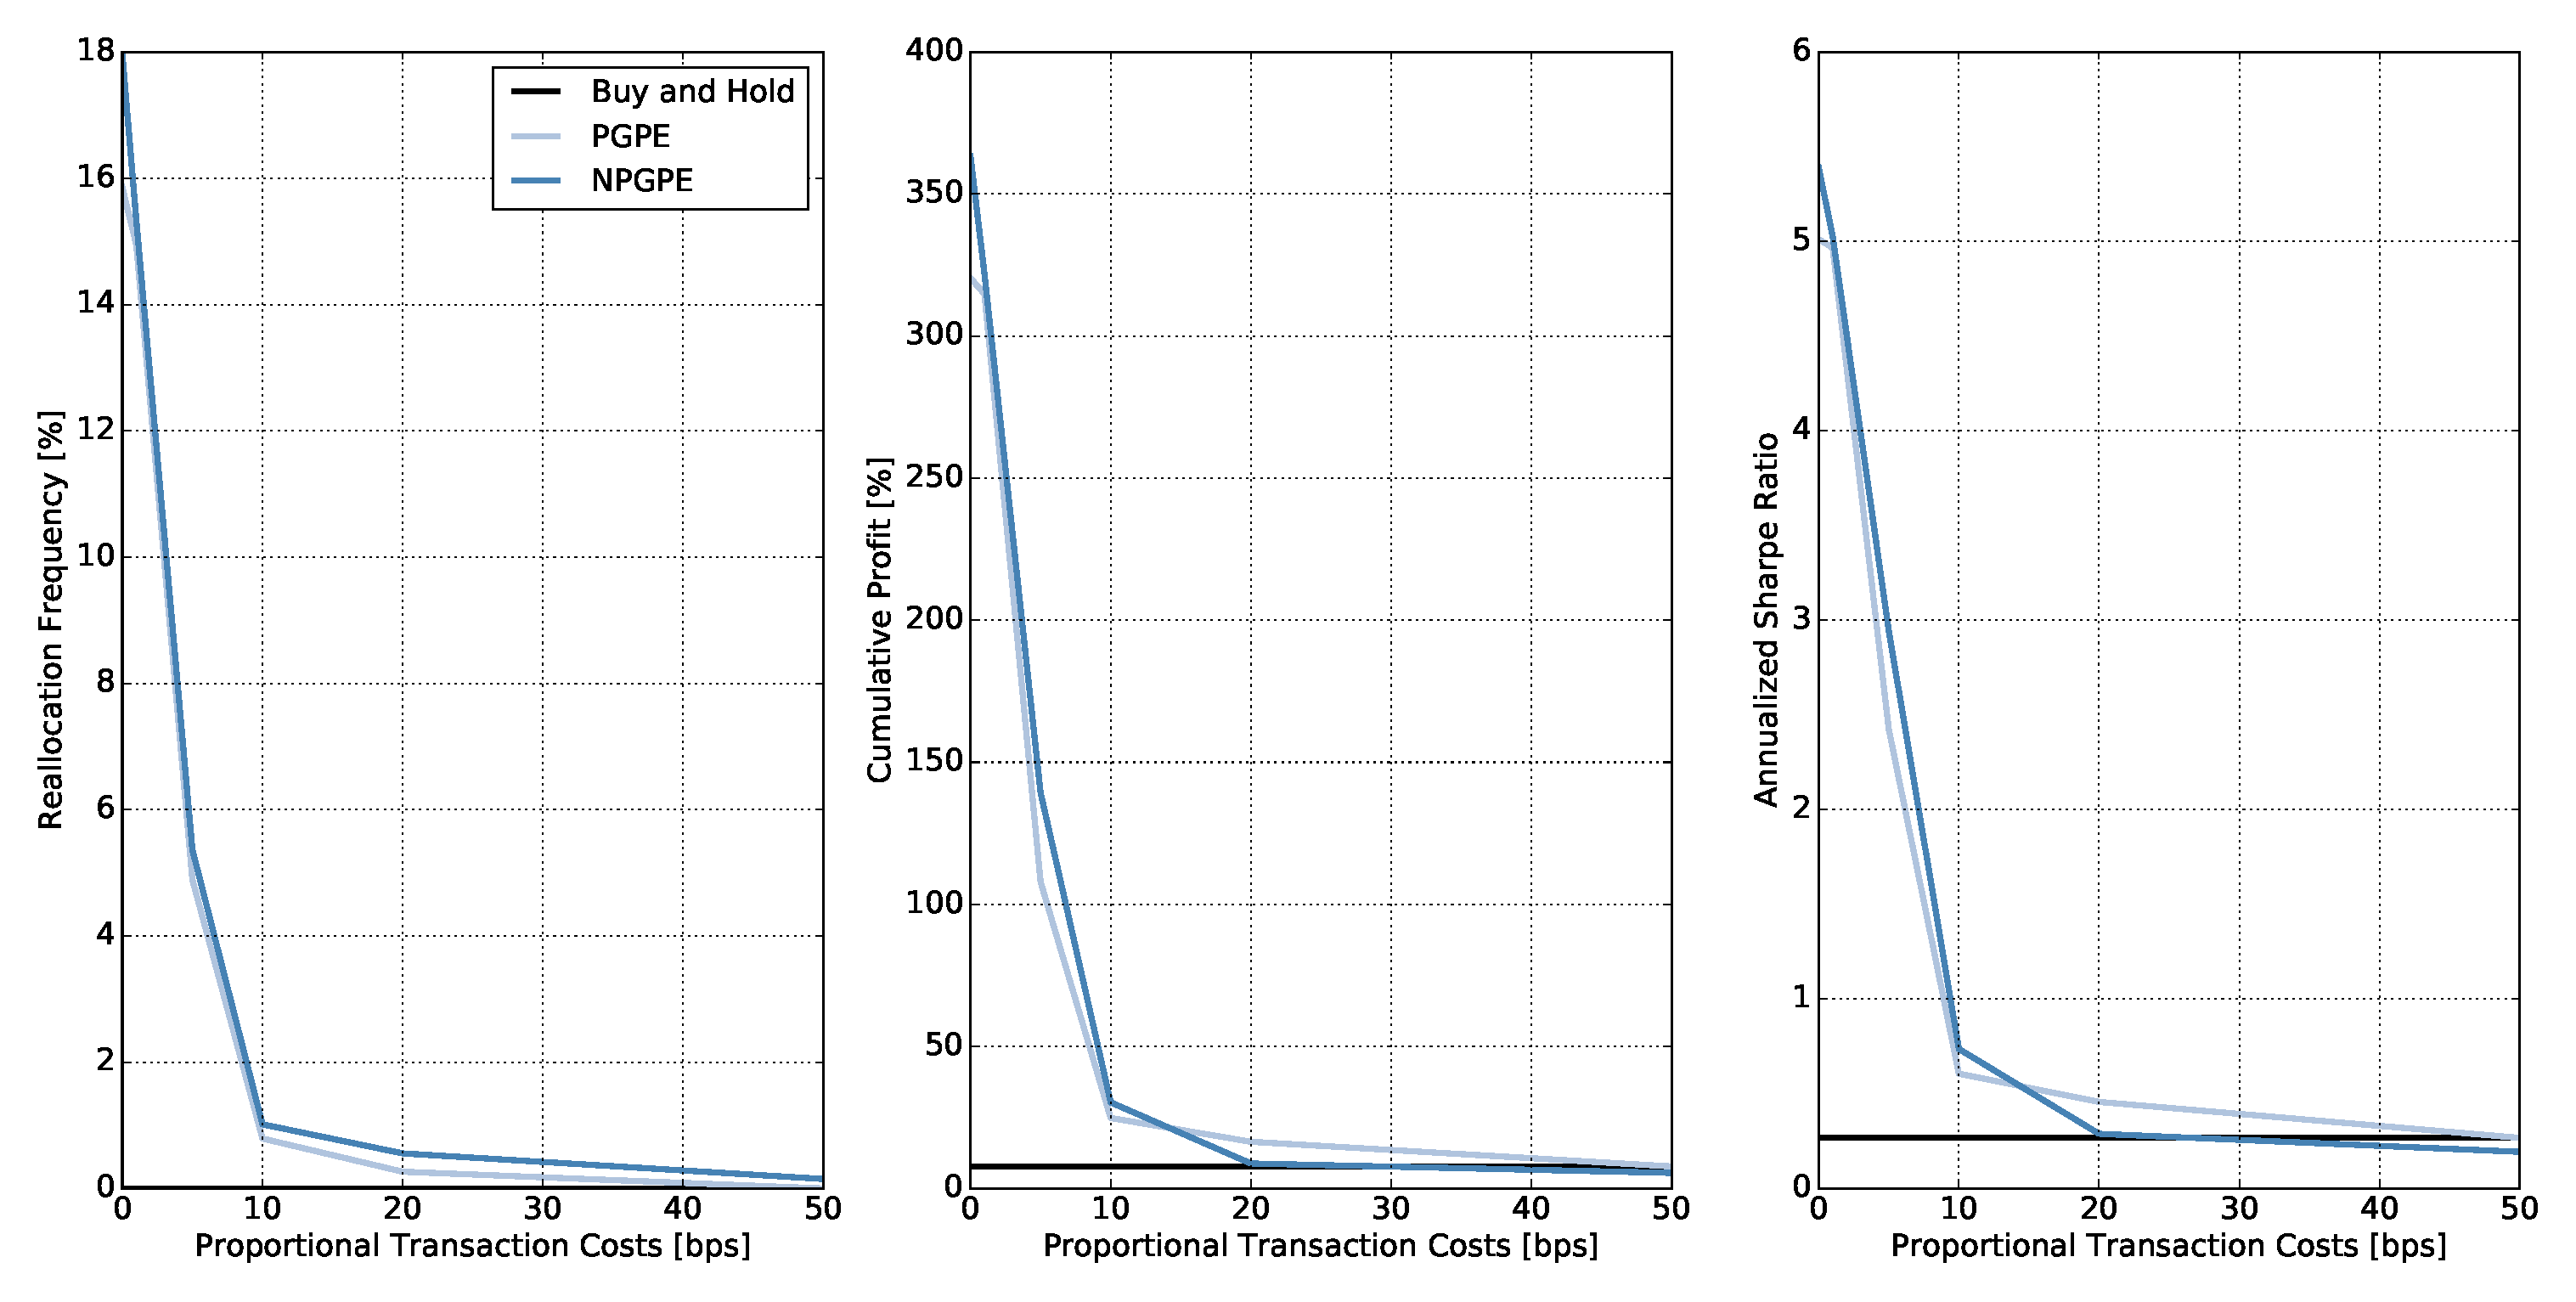
\includegraphics[height=3cm,width=0.8\textwidth]{Images/6_2_impact_transaction_costs}
%\end{figure}
%\begin{figure}[t!]
%	\centering
%	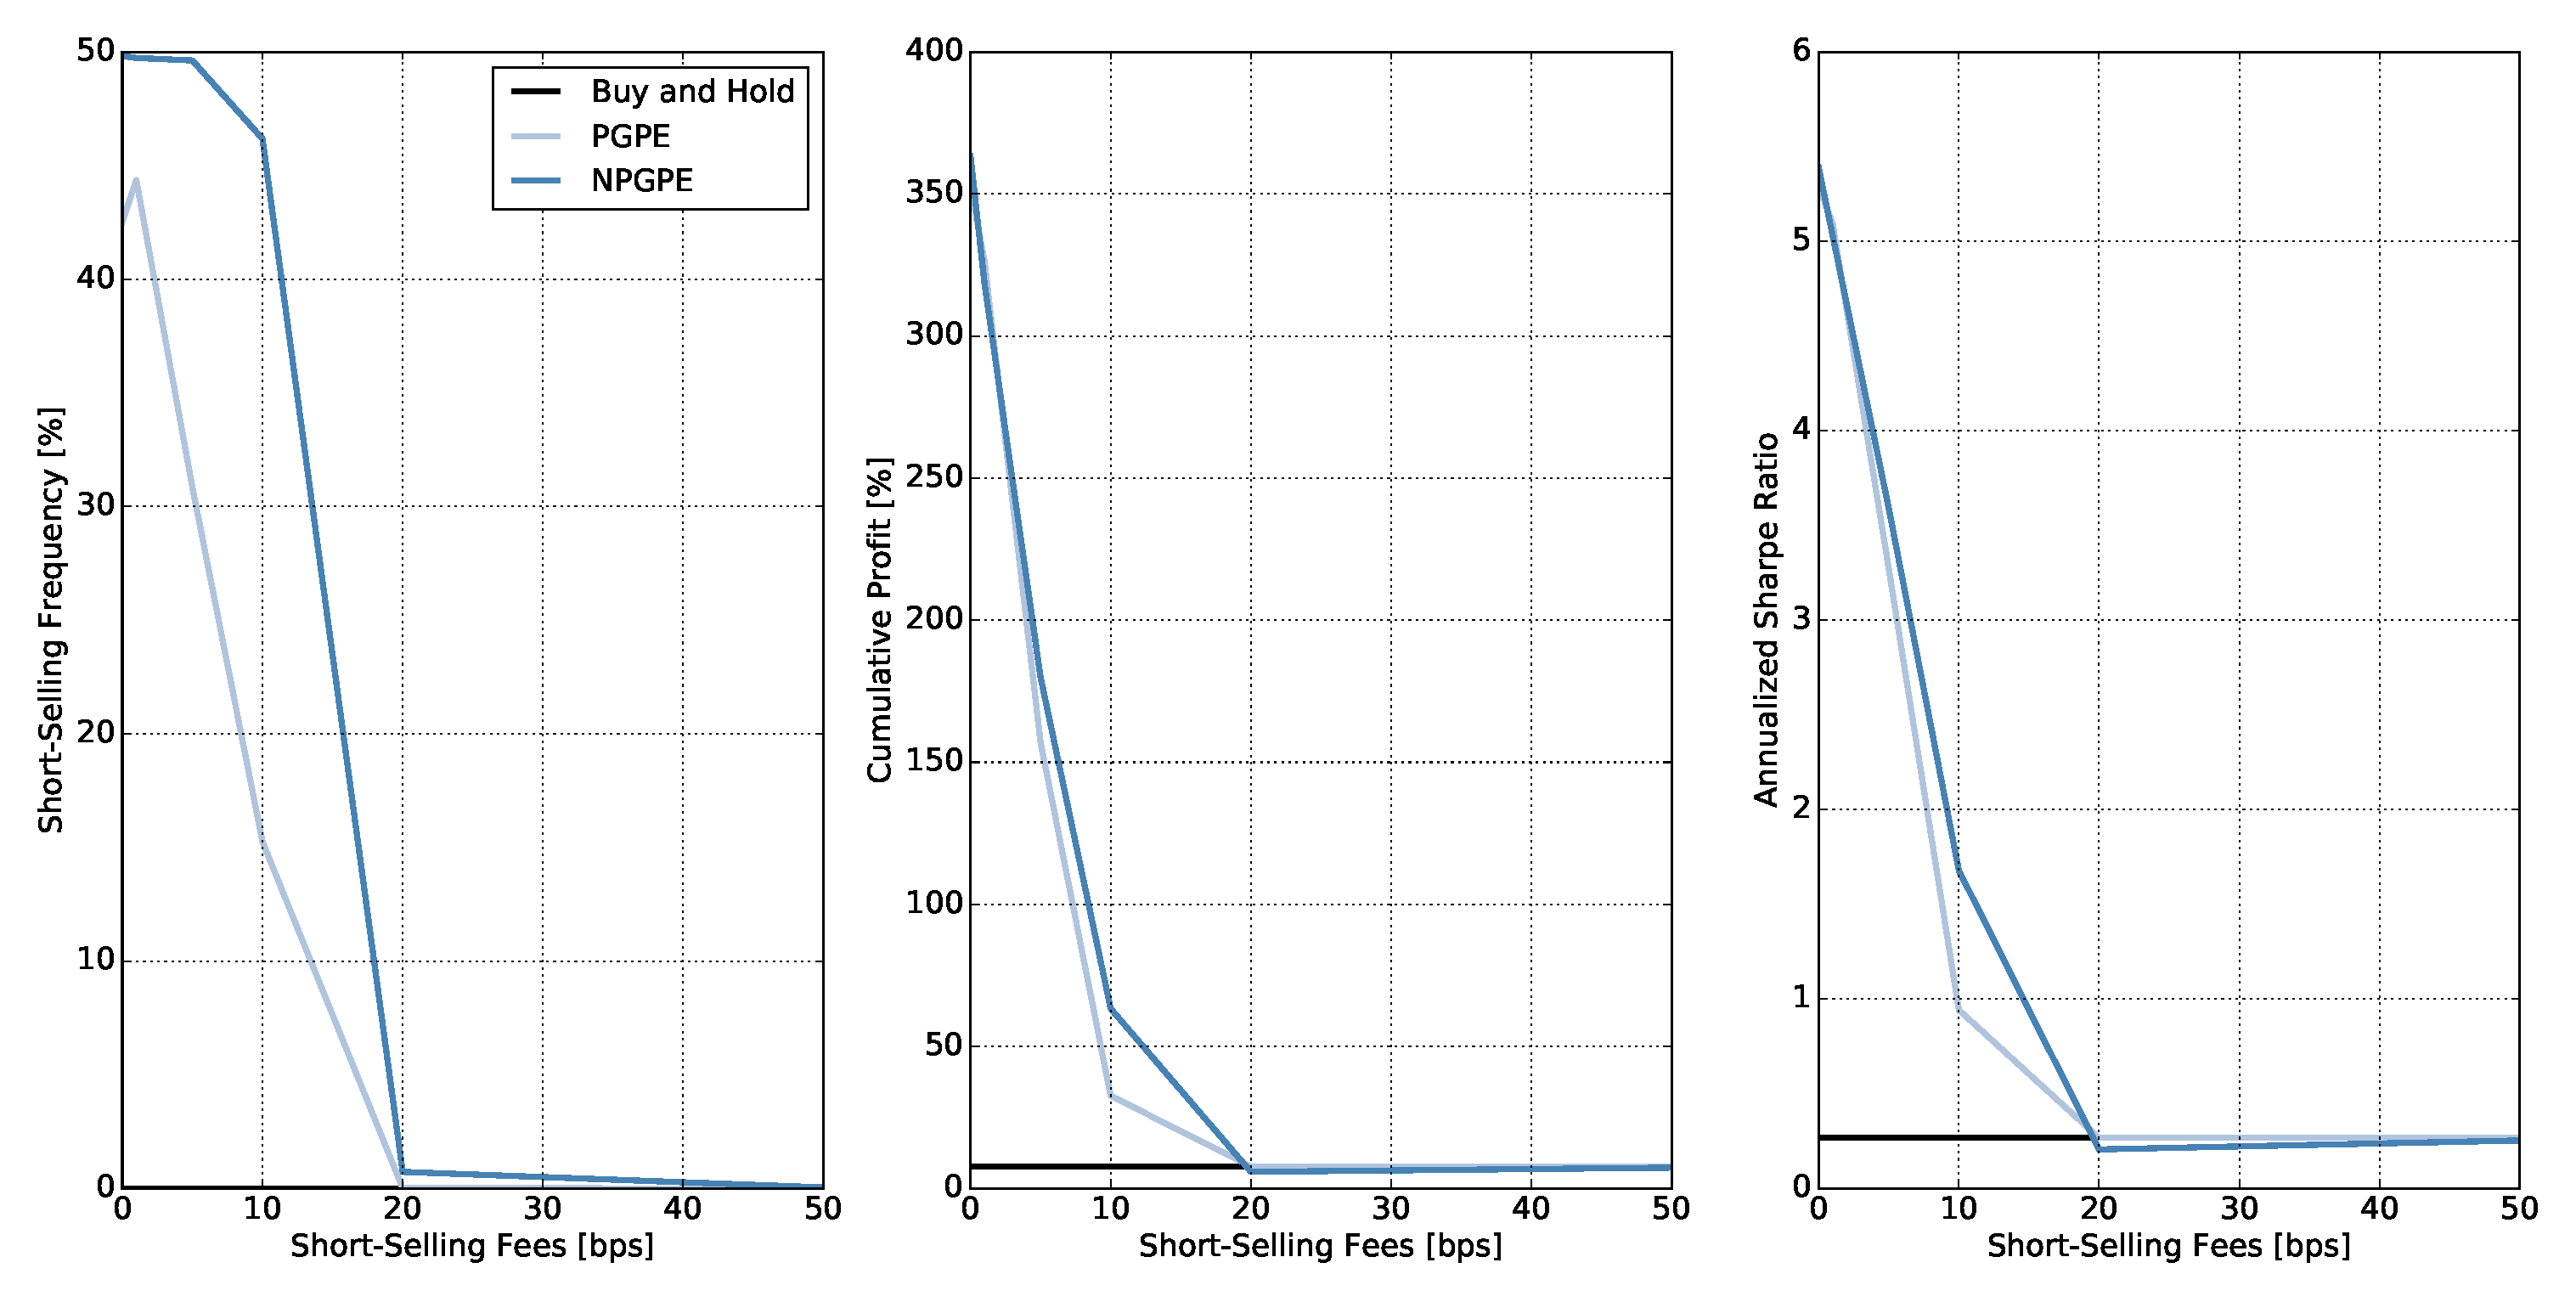
\includegraphics[height=3cm,width=0.8\textwidth]{Images/6_3_impact_short_selling_fees}
%\end{figure}
%\end{frame}
%
%\begin{frame}{Not So Fast}
%
%	\onslide<1->{
%	\begin{columns}
%	\begin{column}{0.6\textwidth}
%	   \begin{alertblock}{Insuccess on Historical Data}
%	   Successfully applying these RL algorithms to historical data is much more challenging
%	   \begin{enumerate}
%	   		\item Fail to converge
%	   		\item The strategies learned are not profitable
%	   \end{enumerate}
%	   \end{alertblock}
%	\end{column}
%	\begin{column}{0.4\textwidth}
%	    \begin{center}
%	     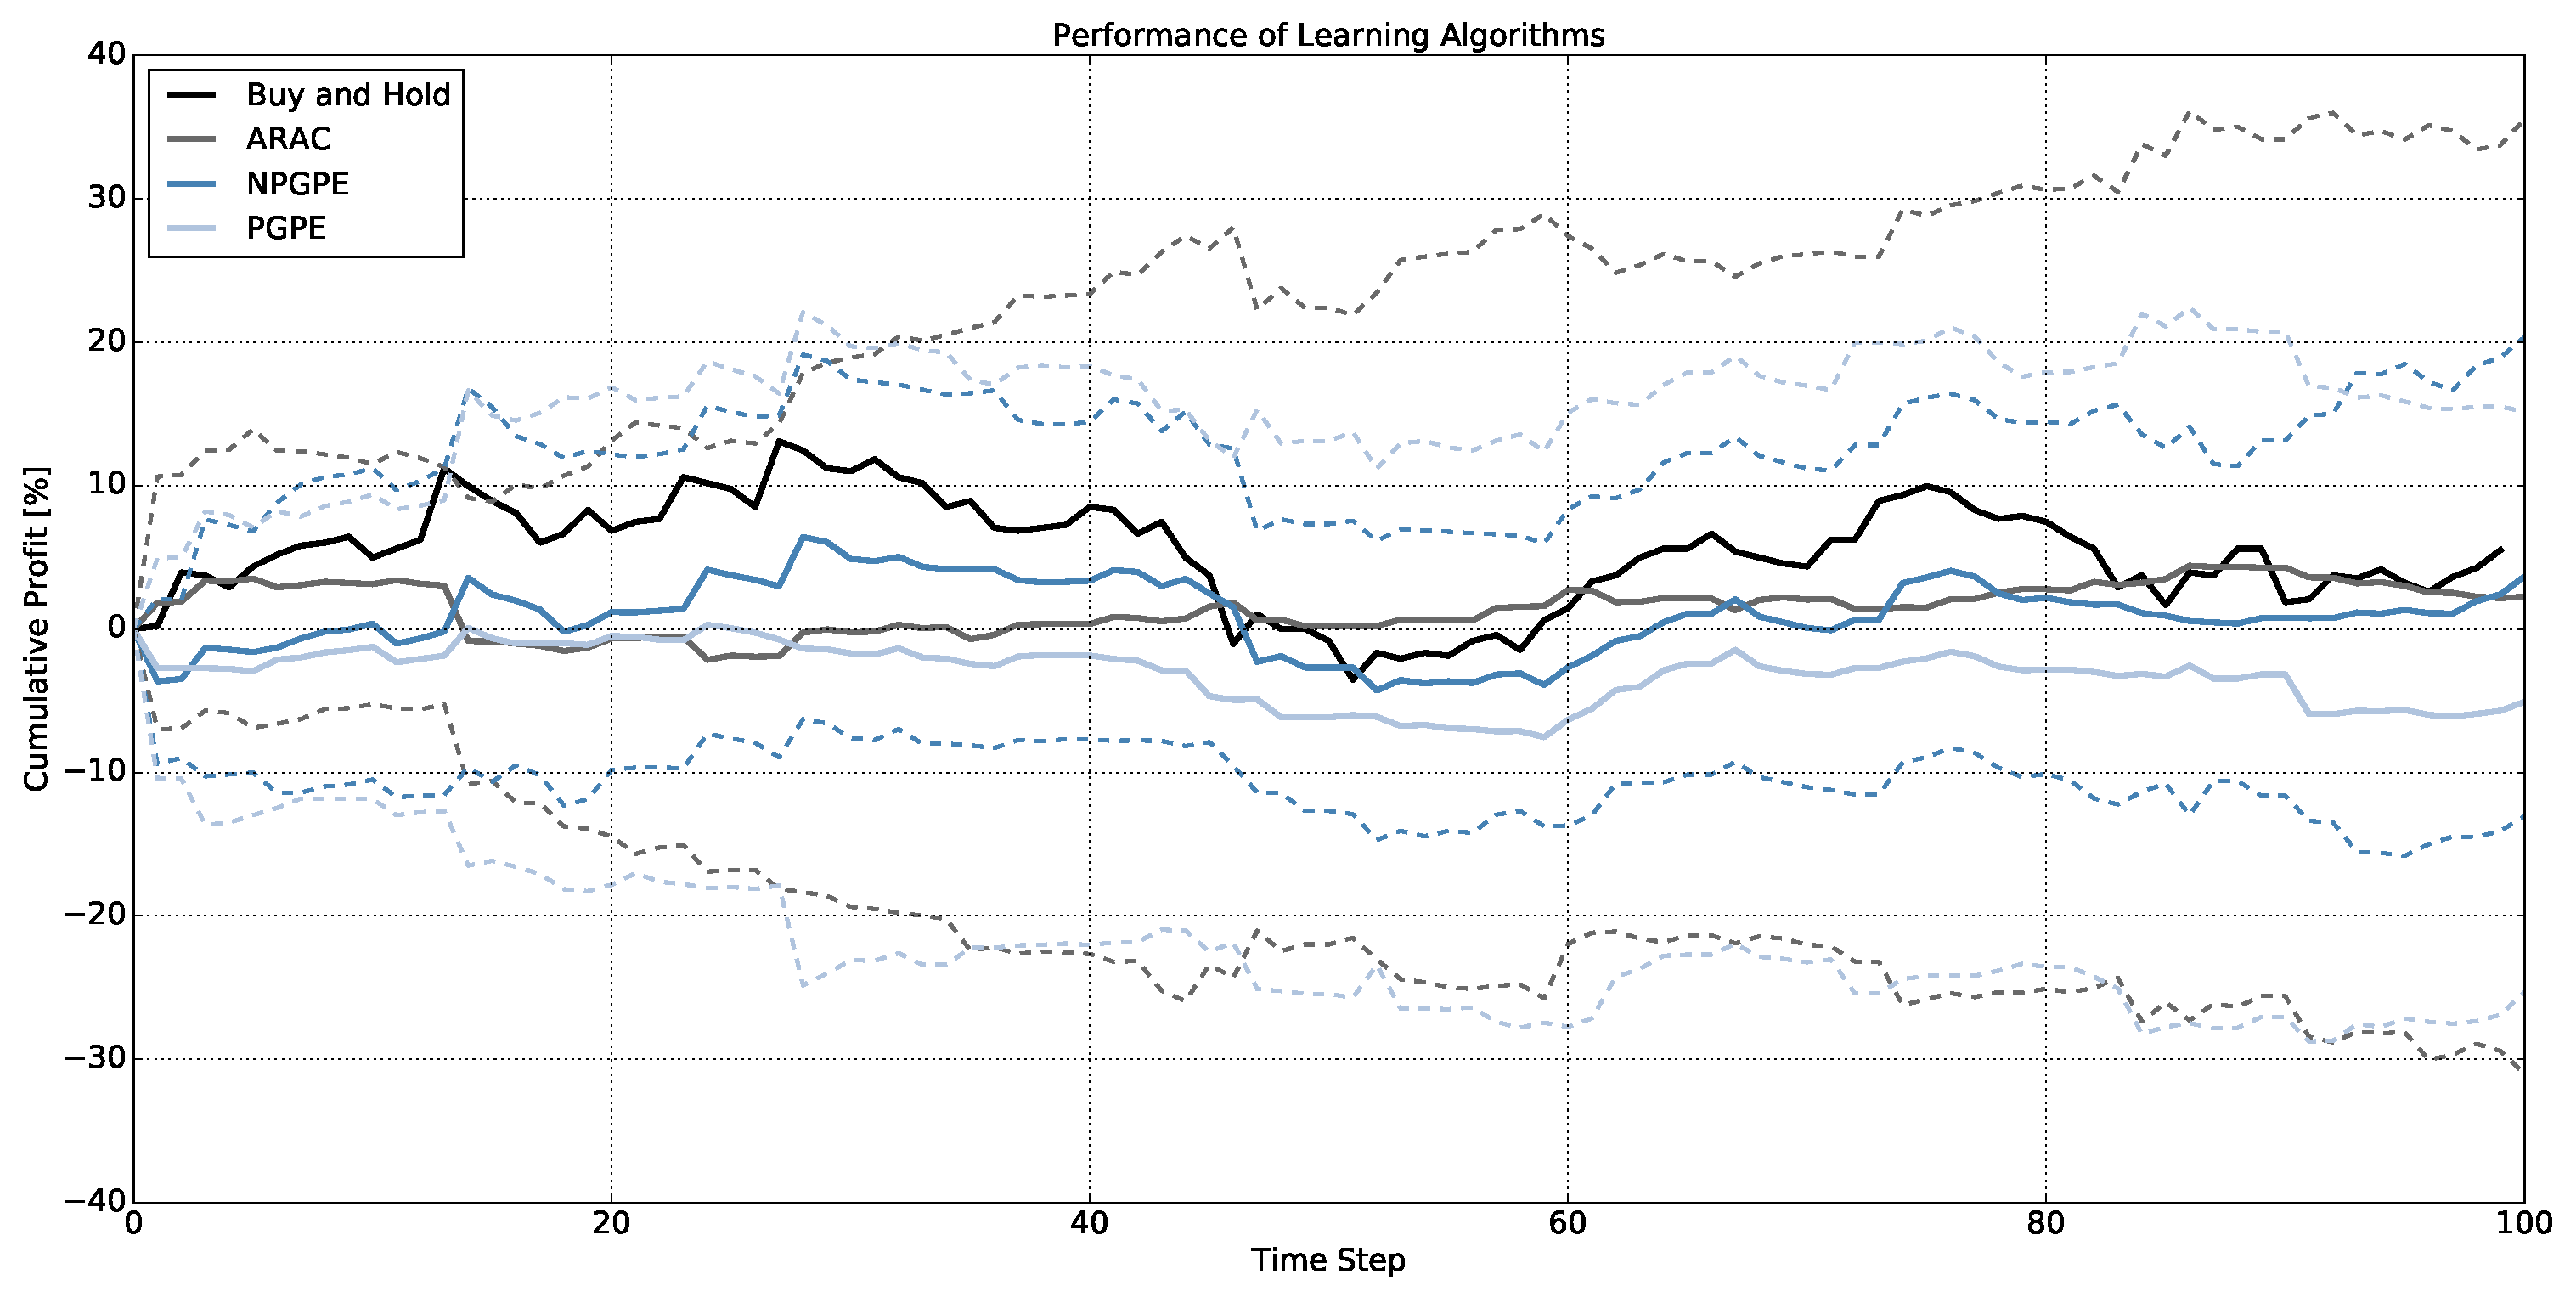
\includegraphics[width=1\textwidth]{Images/8_9_single_hist_neutral_performance}
%	     \end{center}
%	\end{column}
%	\end{columns}
%	}
%	
%	\onslide<2->{	
%	\begin{block}{Possible Explanations}
%		\begin{enumerate}
%			\item<2-> \textbf{Low signal-to-noise ratio}: extremely difficult to find tradable patterns in markets
%			\item<3-> \textbf{Quality of data}: unlikely to find patterns in daily prices of liquid stocks
%			\item<4-> \textbf{Weak features}: parametric policy must be powerful enough to capture the signal
%			\item<5-> \textbf{Non-stationarity of financial time-series}: a signal needs to be persistent
%		\end{enumerate}
%	\end{block}
%	}


%\section{Conclusions}

\begin{frame}{Conclusions}
	\begin{block}<+->{What Has Been Done}
		\begin{enumerate}
			\item In-depth bibliographical study of state-of-the-art policy gradient algorithms
			\item Innovative contributions to the policy gradient literature
			\item Applied these techniques to find a profitable long-short trading strategy		
 		\end{enumerate}
	\end{block}
	
	\begin{block}<+->{Research Directions}
		\begin{enumerate}
			\item Improve the algorithms performance on historical data
			\item Develop more complex features for the trading strategy
			\item Combine policy gradient algorithms with state-of-the-art deep learning techniques
			\item RL framework is versatile and can be applied to other financial decision problems
		\end{enumerate}
	\end{block}
\end{frame}



\begin{frame}[c]{}
  \begin{center}
	  \Huge Thank you for your attention!
  \end{center} 
\end{frame}

%------------------------------------------------------------------------------
% Appendice
%------------------------------------------------------------------------------

\appendix
\backupbegin

\begin{frame}
\frametitle{\refname}
\nocite{*}
\bibliographystyle{acm}
\bibliography{Bibliography/bibliography}
\end{frame}

%\begin{frame}{Markov Decision Processes}
	\begin{block}{Reinforcement Learning}
		General class of algorithms that allow an agent to learn how to behave
		in a stochastic and possibly unknown environment by trial-and-error.
	\end{block}
	
	\begin{block}{Markov Decision Process (MDP)}
		stochastic dynamical system specified by $<\S, \A, \calP, \calR, \gamma>$
		\begin{enumerate}
			\item $(\S, \calS)$ is a measurable state space
			\item $(\A, \calA)$ is a measurable action space
			\item $\calP: \S \times \A \times \calS \to \R$ is a Markov transition kernel
			\item $\calR: \S \times \A \to \R$ is a reward function
			\item $0 < \gamma < 1$ is the discount factor.
		\end{enumerate}
	\end{block}
\end{frame}


\begin{frame}{Policy Gradient Theorem: Statement and Proof}

	\begin{block}{Policy Gradient Theorem}
	Let $\pi_\theta$ be a differentiable policy. For the gradient of the average reward is 
	\begin{equation*}
		\nabla_\theta \rho(\theta) =
		\E[\substack{S \sim d^\theta\\A \sim \pi_\theta}]{\nabla_\theta\log
		\pi_\theta(S,A) Q_{\theta}(S, A)}
	\end{equation*}
	where $d^\theta$ is the stationary distribution of the Markov chain induced by $\pi_\theta$. 
	\end{block}
	\textbf{Proof}\\
	\scalebox{0.8}{%
	$\nabla_\theta V_\theta(s) = \nabla_\theta \int_{\A} \pi_\theta(s,a) Q_\theta(s,a) da = \int_{\A} \left[ \nabla_\theta \pi_\theta(s,a) Q_\theta(s,a) + \pi_\theta(s,a) \nabla_\theta Q_\theta(s,a)\right] da$
	} 
	\scalebox{0.8}{%
	$\nabla_\theta Q_\theta(s,a) = \nabla_\theta \left[ \calR(s,a) - \rho_\theta + \int_{\S} \calP(s,a,s') V_\theta(s') ds' \right] = -\nabla_\theta \rho_\theta + \int_{\S} \calP(s,a,s') \nabla_\theta V_\theta(s') ds'$
		} 
		\scalebox{0.8}{%
	$\nabla_\theta V_\theta(s) = \int_{\A} \nabla_\theta \pi_\theta(s,a) Q_\theta(s,a) da - \nabla_\theta \rho_\theta + \int_\A \pi_\theta(s,a) \int_{\S} \calP(s,a,s') \nabla_\theta V_\theta(s') ds'$
		} 
		\scalebox{0.8}{%
	$\int_{\S} d^\theta(s) \int_{\A} \pi(s,a) \int_{\S} \calP(s,a,s') \nabla_\theta V(s') ds' da ds = \int_{\S} d^\theta(s) \nabla_\theta V_\theta(s) ds$
		} 
		\scalebox{0.8}{%
	$\nabla_\theta \rho_\theta = \int_{\S} d^\theta(s) \int_{\A} \nabla_\theta \pi_\theta(s,a) Q_\theta(s,a) da ds = \int_{\S} d^\theta(s) \int_{\A} \pi_\theta(s,a) \nabla_\theta \log\pi_\theta(s,a) Q_\theta(s,a) da ds$
	}
\end{frame}



\begin{frame}{Monte-Carlo Policy Gradient: Pseudocode}
	\begin{algorithmic}[1]
		\Require Stochastic policy $\pi_\theta$, Initial parameters $\theta_0$, learning rate $\{\alpha_k\}$
		\Ensure Approximation of the optimal policy $\pi_{\theta^*} \approx \pi_*$
		\Repeat
			\State Sample $M$ trajectories $h^{(m)} = \{(s_t^{(m)}, a_t^{(m)}, r_{t+1}^{(m)})\}_{t = 0}^{T^{(m)}}$ under policy $\pi_{\theta_k}$   
			\State Approximate policy gradient 
			\begin{equation*}
				\nabla_\theta J(\theta_k) \approx \frac{1}{M} \sum_{m=0}^M
				 \sum_{u=0}^{T^{(m)}-1} \nabla_\theta\log \pi_{\theta_k} \left(s_u^{(m)}, a_u^{(m)}\right) 
				 \sum_{v \geq u}^{T^{(m)}-1} \gamma^{v-u} r_{v+1}^{(m)}   
			\end{equation*}
			\State Update parameters using gradient ascent $\theta_{k+1} = \theta_k + \alpha_k \nabla_\theta J(\theta_k)$
			\State $k \leftarrow k + 1$
		\Until{converged}
	\end{algorithmic}
\end{frame}


\begin{frame}{Episodic PGPE Algorithm: Pseudocode}
	\begin{algorithmic}[1]
		\Require Controller $F_\theta$, hyper-distribution $p_\xi$, initial guess $\xi_0$, learning rate $\{\alpha_k\}$
		\Ensure Approximation of the optimal policy $F_{\xi^*} \approx \pi_*$
		\Repeat
			\For {$m = 1, \ldots, M$}
				\State Sample controller parameters $\theta^{(m)} \sim p_{\xi_k}$ 
				\State Sample trajectory $h^{(m)} = \{(s_t^{(m)}, a_t^{(m)}, r_{t+1}^{(m)})\}_{t = 0}^{T^{(m)}}$ under policy $F_{\theta^{(m)}}$
			\EndFor
			\State Approximate policy gradient 
		  		\begin{equation*}
		  		\nabla_\xi J(\xi_k) \approx \frac{1}{M} \sum^{M}_{m=1} \nabla_\xi \log p_\xi\left(\theta^{(m)}\right) \left[G\left(h^{(m)}\right)-b\right] 
		  		\end{equation*}
		  		
			\State Update hyperparameters using gradient ascent $\xi_{k+1} = \xi_k + \alpha_k \nabla_\xi J(\xi_k)$
			\State $k \leftarrow k + 1$
		\Until{converged}
	\end{algorithmic}
\end{frame}

\begin{frame}{Natural PGPE Algorithm: Pseudocode}
	\begin{algorithmic}[1]
		\Require Controller $F_\theta$, hyper-distribution $p_\xi$, initial guess $\xi_0$, learning rate $\{\alpha_k\}$
		\Ensure Approximation of the optimal policy $F_{\xi^*} \approx \pi_*$
		\Repeat
			\State Observe current state $s_k$
			\State Draw $\zeta_k \sim \calN(0, I_n)$
			\State Compute controller parameters $\theta_k = \mu_k + \Gamma^T \zeta_k$
			\State Perform action $a_k = F_{\theta_k}(s_k)$ and receive reward $r_{k+1}$
			\State Update average reward estimate $\widehat{\rho}_{k+1} = \widehat{\rho}_{k} + \alpha_k (r_{k+1} - \widehat{\rho}_{k})$
			\State Compute natural policy gradients
				\begin{equation*}
					\begin{split}
						\widetilde{\nabla}_\mu \log p_{\xi_k}(\theta_k) = \theta_k - \mu_k \;\;\;\;\;
						\widetilde{\nabla}_\Gamma \log p_{\xi_k}(\theta_k) = \left(\triu(\zeta_k \zeta_k^T) - \frac{1}{2} \diag(\zeta_k \zeta_k^T) - \frac{1}{2} I \right) \Gamma
					\end{split}
				\end{equation*}
			\State Update eligibility trace $e_{k} = \lambda e_{k-1} + \nabla_\xi \log p_{\xi_k}(\theta_k)$
			\State Update hyper-parameters $\xi_{k+1} = \xi_k + \alpha_k (r_{k+1} - \widehat{\rho}_{k}) e_k$
			\State $k \leftarrow k + 1$
		\Until{converged}
	\end{algorithmic}
\end{frame}



\begin{frame}{Experiment on Synthetic Asset}
	The synthetic asset price is given by
	\begin{equation*}
		Z_t = \exp\left(\frac{z_t}{\max_t z_t - \min_t z_t}\right)
	\end{equation*}
	where $\{z_t\}$ is a random walk with autoregressive trend $\{\beta_t\}$
		\begin{equation*}
			\begin{split}
				z_t &= z_{t-1} + \beta_{t-1} + \kappa \epsilon_t\\
				\beta_t &= \alpha \beta_{t-1} + \nu_t\\
			\end{split}
		\end{equation*}
	The policy used for the PGPE and the NPGPE algorithms is 
	\begin{equation*}
		F_\theta(s) = \sign(\theta \cdot s)
	\end{equation*}
	where
	\begin{equation*}
		\theta \sim \calN(\mu, \diag(\sigma))
	\end{equation*}  
\end{frame}

\begin{frame}[c]{PyBrain's Architecture for a RL Problem}
\begin{figure}[t!]
	\centering
	\begin{tikzpicture}[node distance = 6em, auto, thick]
		\node (rect) at (0,0) [draw,thick,minimum width=8cm,minimum height=6cm] (Experiment) {};
		\node (rect) at (0,1.4) [draw,thick,minimum width=6cm,minimum height=2cm] (Task) {};
		\node (rect) at (0,1.4) [draw,thick,minimum width=3cm,minimum height=1cm] (Environment) {\texttt{Environment}};
		\node (rect) at (0,-1.4) [draw,thick,minimum width=6cm,minimum height=2cm] (Agent) {};
		\node (rect) at (-1.9,-1.4) [draw,thick,minimum width=1.6cm,minimum height=1cm] (Critic) {\texttt{Critic}};
		\node (rect) at (1.9,-1.4) [draw,thick,minimum width=1.6cm,minimum height=1cm] (Learner) {\texttt{Learner}};
		\node (rect) at (0,-1.4) [draw,thick,minimum width=1.6cm,minimum height=1cm] (Actor) {\texttt{Actor}};
		
		\draw (-2.8,3.3) node {\texttt{Experiment}};
		\draw (-2.4,2.7) node {\texttt{Task}};
		\draw (0.8,0) node {\texttt{Action}};
		\draw (-2.25,1.7) node {\texttt{State}};	
		\draw (2.7,0) node {\texttt{Reward}};
		\draw (-2.4,-2.7) node {\texttt{Agent}};
	
		\path [line] (Task.180) --++ (-0.5cm,0cm) |- node [near start]{\texttt{Observation}} (Agent.180);
		\path [line] (Task.0) --++ (+0.5cm,0cm) |- (Agent.0);
		\draw[line] (Environment.180) -- (Task.180);
		\draw[line] (Agent.90) -- (Task.270); 
	\end{tikzpicture}
\end{figure}	
\end{frame}

\begin{frame}[c]{Agent-Environment Interaction in C++}
	\begin{block}{Adapting PyBrain's Architecture}
		\begin{enumerate}
			\item Defined standard interfaces via pure abstract classes
			\item Achieved modularity via polymorphic composition
		\end{enumerate}
	\end{block}
	
	\begin{figure}[h]
		\centering
		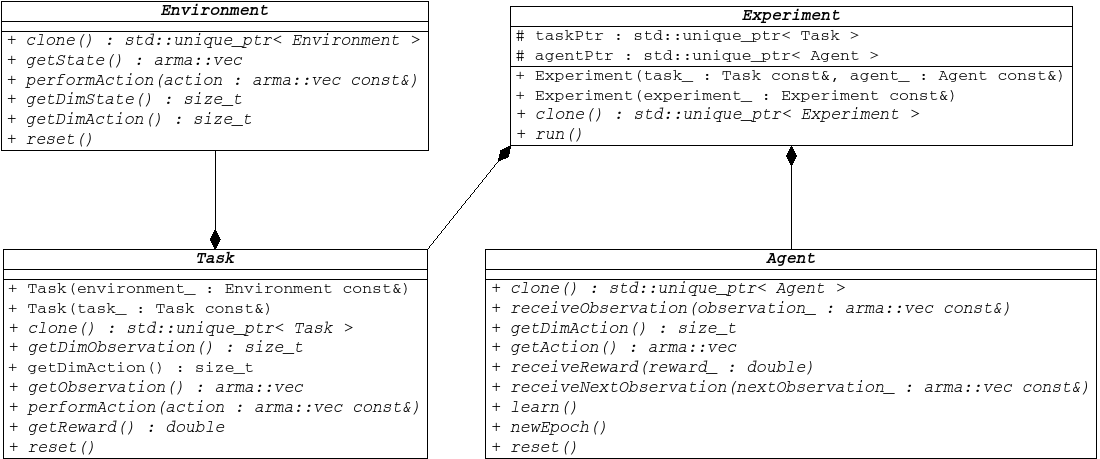
\includegraphics[width=0.8\framewidth]{Images/AgentEnvironmentInteractionReduced}
	\end{figure}
\end{frame}

\begin{frame}[c]{Agent's Architecture in C++}
	\begin{figure}[h]
		\centering
		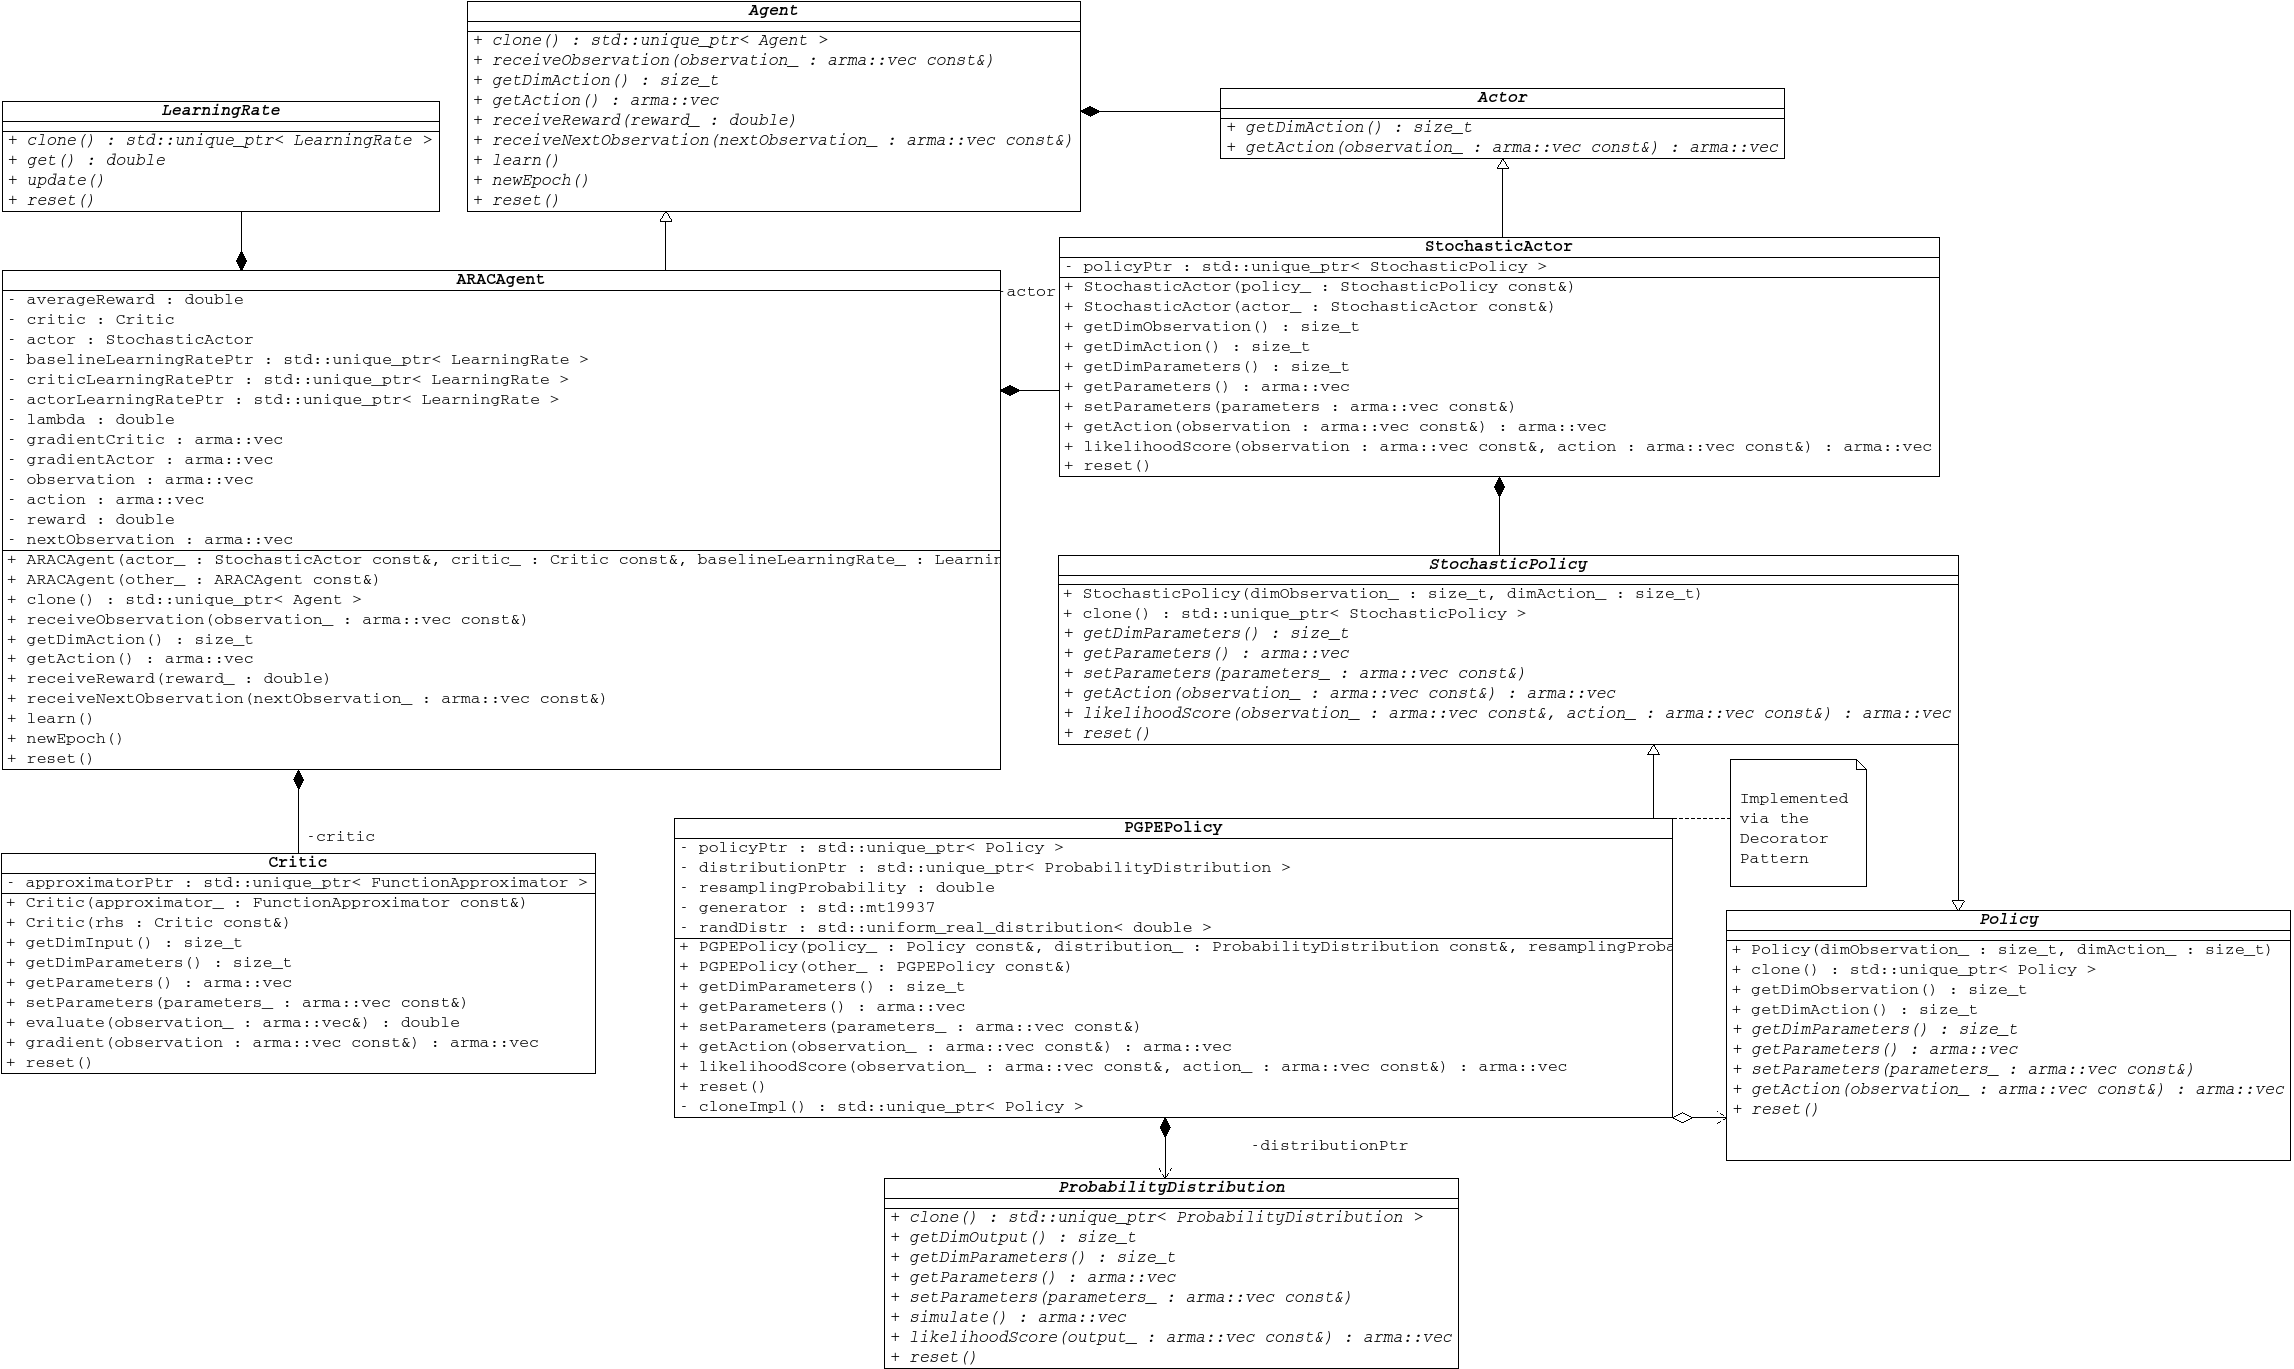
\includegraphics[width=0.8\framewidth]{Images/agent_reduced}
	\end{figure}
\end{frame}

\begin{frame}[c]{Execution Pipeline}
	\begin{block}{\texttt{experiment\_launcher.py}}
		\begin{enumerate}
			\item Program execution is handled by a Python script
			\item Responsible for analyzing the output of the C++ engine
		\end{enumerate}
	\end{block}

	\begin{figure}
		\centering
		\resizebox{0.8\framewidth}{!}{%
		\begin{tikzpicture}[node distance = 6em, auto, thick]
			\node (rect) at (-9.5,-2) [DimGray,draw,thick,minimum width=3cm,minimum height=3cm] (generate_synthetic_series) {};
			\node (rect) at (0,0) [DimGray,draw,thick,minimum width=15cm,minimum height=10cm] (experiment_launcher) {};
			\node (rect) at (+9,-2) [IndianRed,draw,thick,minimum width=2cm,minimum height=3cm] (convergence) {};
			\node (rect) at (+9,+2) [IndianRed,draw,thick,minimum width=2cm,minimum height=3cm] (performance) {};
			\node (rect) at (-6,2) [IndianRed,draw,thick,minimum width=2cm,minimum height=3cm] (input) {};
			\node (rect) at (-6,-2) [IndianRed,draw,thick,minimum width=2cm,minimum height=3cm] (synthetic) {};
			\node (rect) at (-2,0) [SteelBlue, draw,thick,minimum width=4cm,minimum height=8cm] (main_thesis) {};
			\node (rect) at (2,2) [IndianRed,draw,thick,minimum width=2cm,minimum height=3cm] (output) {};
			\node (rect) at (2,-2) [IndianRed,draw,thick,minimum width=2cm,minimum height=3cm] (debug) {};
			\node (rect) at (5.5,0) [DimGray,draw,thick,minimum width=3cm,minimum height=3cm] (postprocessing) {};
			
			\draw (0,5.5) node {\lstinline{experiment_launcher.py}};
			\draw (-9.5,0) node {\lstinline{generate_synthetic_series.py}};
			\draw (-6,-4) node {\lstinline{synthetic.csv}};
			\draw (-7.8,4) node {\lstinline{Single_Synth_RN_P0_F0_S0_N5.pot}};	
			\draw (5.5,2) node {\lstinline{postprocessing.py}};
			\draw (2,4) node {\lstinline{output.csv}};
			\draw (2,-4) node {\lstinline{debug.csv}};
			\draw (9.5,4) node {\lstinline{performance.csv}};
			\draw (9.5,-4) node {\lstinline{convergence.csv}};
			\draw (-2,0) node {\lstinline{main_thesis}};	
		
			\draw[line] (generate_synthetic_series.0) -- (synthetic.180);
			\draw[line] (debug.0) -- (postprocessing.180);
			\draw[line] (output.0) -- (postprocessing.180);
			\draw[line] (postprocessing.0) -- (performance.180);
			\draw[line] (postprocessing.0) -- (convergence.180);
			\draw[line] (input.0) -- (main_thesis.135);
			\draw[line] (synthetic.0) -- (main_thesis.225);
			\draw[line] (main_thesis.45) -- (output.180);
			\draw[line] (main_thesis.315) -- (debug.180);
		\end{tikzpicture}}
	\end{figure}
\end{frame}

\backupend

\end{document}
